\documentclass{article}
\usepackage{graphicx} % Required for inserting images
\usepackage[utf8]{inputenc} % allow utf-8 input
\usepackage[T1]{fontenc}    % use 8-bit T1 fonts
\usepackage{hyperref}       % hyperlinks
\usepackage{url}            % simple URL typesetting
\usepackage{booktabs}       % professional-quality tables
\usepackage{amsfonts}       % blackboard math symbols
\usepackage{nicefrac}       % compact symbols for 1/2, etc.
\usepackage{microtype}      % microtypography
\usepackage{xcolor}         % colors
\usepackage[utf8]{inputenc} % allow utf-8 input
\usepackage[T1]{fontenc}    % use 8-bit T1 fonts
\usepackage{hyperref}       % hyperlinks
\usepackage{url}            % simple URL typesetting
\usepackage{booktabs}       % professional-quality tables
\usepackage{amsfonts}       % blackboard math symbols
\usepackage{nicefrac}       % compact symbols for 1/2, etc.
\usepackage{microtype}      % microtypography
\usepackage{xcolor}         % colors
\usepackage{graphicx}
\usepackage{amsmath}
\usepackage[round]{natbib}
\usepackage{amsthm}
\usepackage{xspace}
\usepackage{cleveref}
\usepackage{subcaption}
\usepackage{booktabs}
\usepackage[round]{natbib}
\usepackage{bbding} % for the \CheckmarkBold symbol
\usepackage{pifont}
\usepackage{url} 
\usepackage{hyperref}

\theoremstyle{remark}
\newtheorem{observation}{Observation}

\theoremstyle{definition}
\newtheorem{definition}{Definition}
\newtheorem{example}{Example}

\newcommand{\ttt}[1]{\texttt{#1}\xspace}
\newcommand{\ttti}[1]{\texttt{i}\xspace}
\newcommand{\eg}{e.g.\xspace}


\newtheorem{theorem}{Theorem}[section]
\newtheorem{lemma}[theorem]{Lemma}
\newtheorem{claim}[theorem]{Claim}
\newtheorem{proposition}[theorem]{Proposition}
\newtheorem{corollary}[theorem]{Corollary}
\newtheorem{remark}[theorem]{Remark}
\newcommand{\dpt}[1]{\frac{d#1}{dt}} % Derivative shortcut



\newcommand{\benchmarkname}{T-GRAB\xspace}


\title{floquet_analysis}
\author{Mehrab Hamidi}
\date{May 2025}

\begin{document}

\section{Introduction}

Based on the results discussed above we wished to get more intuition about how some graph model make their decisions by looking at their internal representation. Here, we want to note that there are a few works focus on mechanistic interpretability in GNNs. Very recent work by \citep{el2025towards} tried to mostly do attention visualization for developing an analysis framework for mechanistic interpretability on GNNs. 
We believe that having some intuition and understanding about how internal representations of GNNs look like and how these model making their decision is important and our unified synthetic \textbf{controlled} benchmark gives us a useful tool to evaluate and match the skills required to solve a simple task to learned representations of GNNs. For instance, a GCLSTM model has perfect accuracy \ref{fig:(2,N)_overall} on task $(2, 1)$ \ref{sec:preiodicity} and we hypothesis by looking at the internal structure of this model we have to find some clues about the specification of this task in the internal representation of GCLSTM. Now a natural question of what would be these specification and what should we be exactly looking for would come up. To answer this question we first formalize the introduced periodicity task with Floquet analysis.

\section{Preliminaries}
% https://en.wikipedia.org/wiki/Floquet_theory
Floquet theory is a subbranch of ODEs, relating the class of solutions to periodic linear differential equations of the form:
$$
\dot{x} = A(t) x
$$
with $x \in \mathbb{R}$ and $A(t) \in \mathbb{R}^{n\times n}$ being a piecewise continuous periodic function with period $T$ and defines the state of the stability of solutions. A periodic function, also called a periodic waveform (or simply periodic wave), is a function that repeats its values at regular intervals or periods. 

\begin{definition}
A function $f$ is said to be periodic, if for some non-zero constant $P$, it is the case that:
$$
f(x+P) = f(x)
$$
For all the values $x$ in its domain.
% Let $(T, +)$ be a discrete time index set, and let $X$ be any set (e.g. real numbers, characters in a text, graph snapshots, etc.). A \textbf{signal} is a function 
% \[
% S: T \longrightarrow X
% \]
% We say $S$ is \textbf{Periodic} with period (positive) $\tau \in T $ if
% \[
% \forall t \in T: \quad S(t+\tau) = S(t)
% \]
% % Let \( S \) be a structure defined over a domain, such as a function, sequence, graph, or pattern. We say that \( S \) is \emph{periodic} with period \( P \neq 0 \) if there exists an operation (such as a shift, translation, or transformation) denoted by \( x \mapsto x + P \) such that
% % \[
% % S(x + P) = S(x)
% % \]
% % holds for all valid inputs or positions \( x \) in the domain of \( S \).

% % The smallest positive value \( P \) satisfying this condition is called the \emph{fundamental period} of \( S \).
\end{definition} \label{def:periodicity}

Note that definition \ref{def:periodicity} is general since $X$ can be any desired domain. Now inspired by our periodicity tasks \ref{sec:preiodicity}, fix a finite ordered list (alphabet) set of $N$ patterns/graphs $\mathcal{G} = \{G_1, G_2, \ldots, G_N\} \subset X$ and and integer block-length $k \geq 1$ we define a task-signal:
\[
S_{\mathcal{G}, K}: \mathbb{N} \rightarrow X, \quad S_{\mathcal{G}, K} = G_{(\lfloor t/K\rfloor \bmod N) + 1}
\]
Clearly $S_{\mathcal{G}, K} (t + \tau) = S_{\mathcal{G}, K} (t)$ with $\tau = NK$.
So $S_{\mathcal{G}, K}$ is $\tau$-periodic.\\
To make periodicity part of the specification, introduce the relation
\(\mathcal{R}\subseteq T\times T\) defined by
\[
  (t,i)\in\mathcal{R}
  \quad\Longleftrightarrow\quad
  S(t+i)=S(i).
\]
Then the 4‐tuple
\[
  \Theta
  = \bigl(\,\mathcal{G},\,k,\,\tau,\,\mathcal{R}\bigr)
\]
completely specifies the periodic task.


\begin{theorem}
    The following two specifications are equivalent:
\begin{enumerate}
  \item $(X,T,S,\tau)$ with \(S(t+\tau)=S(t)\).  
  \item $(\mathcal{G},k,\tau,\mathcal{R}\bigr)$ with
  \(\tau=N\,k\) and
  \(\;S(t)=G_{(\lfloor t/k\rfloor\bmod N)+1},\;\mathcal{R}=\{(t,i):S(t+i)=S(i)\}.\)
\end{enumerate}
\end{theorem}

\begin{proof}
    \emph{$(1)\Rightarrow (2)$} Given a $\tau$ periodic $S$, let \(\mathcal{G}\) be its sequence of \(N\) distinct values in one period, in the order they first appear.  If each value appears in contiguous blocks of length \(k=\tau/N\), then one recovers the pattern‐block form.  The shift‐relation \(\mathcal{R}\) follows immediately from periodicity.

    \emph{$(1)\Rightarrow (2)$}
    Given \((\mathcal{G},k,\tau)\) with \(\tau=N\,k\), define \(S\) by \(\;S(t)=G_{(\lfloor t/k\rfloor\bmod N)+1}\).  Then obviously \(S(t+\tau)=S(t)\), and the relation \(\mathcal{R}\) enforces Definition~\ref{def:periodicity}.
\end{proof}

IF a graph sequence model like GCLSTM achieves perfect accuracy on the $(\mathcal{G}, k)$-task, it must internally encode enough information to reconstruct one of the equivalent above specifications. In practice, we want to test this hypothesis by probing the hidden-cell dynamics for Floquet modes at different frequencies. Failure to find stable undamped modes at those frequencies-but instead only decaying or noisy components-indicates the model has \textbf{not} a pure modulo-$\tau$ counter, but rather is repeatedly \emph{re-encoding} the current graph phase and allowing that signal to decay. Which our experimental results in the following section showcase the failure mode. Specifically we wish to undestand how a GCLSTM internally represents a strictly periodic task (e.g. "$A,A,B,B, \dots$". 





\section{Floquet Analysis}


Recurrent neural networks, such as the GCLSTM, are fundamentally discrete-time dynamical systems. To leverage the powerful analytical tools of continuous-time systems, particularly for stability analysis of periodic tasks, it is necessary to establish a continuous-time representation. This section demonstrates a formal procedure for this conversion. 

\begin{itemize}
    \item We derive the continuous-time limit of the GCLSTM's state update rule, resulting in a non-linear Ordinary Differential Equation (ODE). \ref{seq:step1}
    \item We linearize this non-linear ODE around a periodic reference trajectory. This procedure yields a linear, time-varying system of the form $\dpt{z} = A(t)z$, which is amenable to Floquet theory. \ref{seq:step2}
    \item We formally define the Monodromy matrix for this system. \ref{seq:step3} 
    \item We provide a rigorous framework for analyzing the stability of periodic solutions learned by GCLSTMs. \ref{seq:step4}
\end{itemize}



\subsection{From Discrete to Continuous Dynamics} \label{seq:step1}

The core of a GCLSTM is its discrete state update equation. Our first objective is to find a continuous-time ODE whose solution at integer time steps approximates the discrete sequence generated by the GCLSTM. This is achieved by taking the continuous-time limit.

\begin{definition}[GCLSTM State Update]
The discrete state update of a GCLSTM (Definition 1.1) is given by:
\begin{equation}
    s_{t+1} = F(s_t, A_t)
\end{equation} \label{eq:state_update}
where $s_t = (h_t, c_t)$ is the state at integer time $t$ and $F$ represents the collective non-linear operations within the GCLSTM cell.
\end{definition}

To formulate a continuous analogue, we treat the discrete update as an Euler integration step with a step size of $\Delta t = 1$. We can generalize this by re-parameterizing the update rule.


\begin{theorem}[Continuous-Time Limit of GCLSTM]
The discrete dynamics of the GCLSTM in \ref{eq:state_update} can be approximated by a non-linear Ordinary Differential Equation:
\begin{equation}
    \dpt{s(t)} = \mathcal{F}(s(t), A(t))
\end{equation}
where $\mathcal{F}$ is a continuous function derived from the cell dynamics $F$.
\end{theorem}\label{eq:ode_solution_rnn}

\begin{proof}
Let us re-write:
\begin{equation}
    s_{t+1} = s_t + [F(s_t, A_t) - s_t] = s_t + G(s_t, A_t)
\end{equation}
where $G(s_t, A_t) := F(s_t, A_t) - s_t$.

Let us now introduce a continuous time variable $\tau$ and a small time step $\Delta \tau$. We can interpret the discrete update from $t$ to $t+1$ as a single integration step over a time interval of length $\Delta \tau=1$. The equation becomes:
\begin{equation}
    s(\tau + \Delta \tau) = s(\tau) + G(s(\tau), A(\tau))
\end{equation}
where we assume $A(\tau)$ is a piece-wise constant or smoothly interpolated function of time.

Dividing by $\Delta \tau$ and rearranging gives the forward difference quotient:
\begin{equation}
    \frac{s(\tau + \Delta \tau) - s(\tau)}{\Delta \tau} = \frac{G(s(\tau), A(\tau))}{\Delta \tau}
\end{equation}
The standard approach to deriving a continuous model is to consider the limit as the time step approaches zero. In the context of Neural ODEs, we define the continuous dynamics $\mathcal{F}$ such that this limit is well-posed. We define $\mathcal{F}(s, A) := G(s, A)$, effectively scaling the dynamics by $\Delta \tau = 1$.
Taking the limit of the left-hand side as $\Delta \tau \to 0$ yields the definition of the time derivative:
\begin{equation}
    \lim_{\Delta \tau \to 0} \frac{s(\tau + \Delta \tau) - s(\tau)}{\Delta \tau} = \dpt{s(\tau)}
\end{equation}
Thus, we arrive at the continuous-time, non-linear ODE that governs the evolution of the GCLSTM's state:
\begin{equation}
    \dpt{s(t)} = \mathcal{F}(s(t), A(t)) \quad \text{where} \quad \mathcal{F}(s, A) = F(s, A) - s
\end{equation} \label{eq:derived_ode}
The solution to this ODE, $s(t)$, serves as a continuous interpolation of the discrete sequence $\{s_t\}$.
\end{proof}

\subsection{Linearization and Floquet Analysis} \label{seq:step2}

The derived ODE \ref{eq:derived_ode} is non-linear. To apply tools for linear systems, such as Floquet theory, we must linearize the system around a specific solution of interest. Since the task is periodic, we assume there exists a periodic solution.

\begin{definition}[Periodic Reference Solution]
Let the input sequence of graphs be periodic with period $T$, i.e., $A(t+T) = A(t)$. We assume the non-linear system (7) admits a stable periodic solution, denoted $s^*(t)$, such that $s^*(t+T) = s^*(t)$.
\end{definition}

We now analyze the dynamics of small perturbations around this reference solution.

\begin{theorem}[Linearized GCLSTM Dynamics]
The dynamics of a small perturbation $z(t)$ around the periodic solution $s^*(t)$ are governed by the linear, time-varying ODE:
\begin{equation}
    \dpt{z(t)} = A(t) z(t)
\end{equation}
where $A(t)$ is the Jacobian of the continuous dynamics $\mathcal{F}$ evaluated along $s^*(t)$.
\end{theorem}

\begin{proof}
Let $s(t)$ be a solution to Eq. (2) that is slightly perturbed from the reference solution $s^*(t)$. We can write:
\begin{equation}
    s(t) = s^*(t) + z(t)
\end{equation}
where $\|z(t)\|$ is small. Substituting this into Eq. \ref{eq:ode_solution_rnn}:
\begin{equation}
    \dpt{s^*(t)} + \dpt{z(t)} = \mathcal{F}(s^*(t) + z(t), A(t))
\end{equation}
We perform a first-order Taylor expansion of the right-hand side around $s^*(t)$:
\begin{equation}
    \mathcal{F}(s^*(t) + z(t), A(t)) \approx \mathcal{F}(s^*(t), A(t)) + J_{\mathcal{F}}(s^*(t), A(t)) z(t) + O(\|z(t)\|^2)
\end{equation}
where $J_{\mathcal{F}}$ is the Jacobian matrix of $\mathcal{F}$ with respect to its first argument, $s$.

Substituting (11) into (10) and ignoring higher-order terms in $z(t)$:
\begin{equation}
    \dpt{s^*(t)} + \dpt{z(t)} \approx \mathcal{F}(s^*(t), A(t)) + J_{\mathcal{F}}(s^*(t), A(t)) z(t)
\end{equation}
By definition, the reference solution itself satisfies $\dpt{s^*(t)} = \mathcal{F}(s^*(t), A(t))$. These terms cancel, leaving the linear differential equation for the perturbation $z(t)$:
\begin{equation}
    \dpt{z(t)} = A(t) z(t)
\end{equation}
where we define the time-varying matrix $A(t)$ as the Jacobian evaluated along the periodic trajectory:
\begin{equation}
    A(t) := J_{\mathcal{F}}(s^*(t), A(t)) = \frac{\partial \mathcal{F}}{\partial s} \bigg|_{s=s^*(t)}
\end{equation}
Since $s^*(t)$ is T-periodic and we assume $A(t)$ is T-periodic, the matrix $A(t)$ is also T-periodic, i.e., $A(t+T) = A(t)$.
\end{proof}

\subsection{The Monodromy Matrix} \label{seq:step3}
With the T-periodic linear system established, we can now define the monodromy matrix, the central object in Floquet theory.

\begin{definition}[Fundamental Matrix Solution]
The principal fundamental matrix solution, $\Phi(t)$, of the linear system $\dpt{z} = A(t)z$ is the unique matrix solution to the initial value problem:
\begin{equation}
    \dpt{\Phi(t)} = A(t)\Phi(t), \quad \Phi(0) = I
\end{equation}
where $I$ is the identity matrix. The solution to the system for an initial condition $z(0)$ is then $z(t) = \Phi(t)z(0)$.
\end{definition}

\begin{definition}[Monodromy Matrix]
For the T-periodic system $\dpt{z} = A(t)z$, the monodromy matrix, $M$, is the value of the principal fundamental matrix solution after one full period:
\begin{equation}
    M = \Phi(T)
\end{equation}
\end{definition}

\begin{remark}
The monodromy matrix is a constant matrix that maps the perturbation vector from the beginning of a period to its end: $z(T) = M z(0)$. Its eigenvalues, known as Floquet multipliers, determine the stability of the periodic orbit $s^*(t)$. If all eigenvalues of $M$ have a magnitude less than 1, the orbit is asymptotically stable.
\end{remark}

% We have presented a rigorous mathematical framework to bridge the gap between discrete-time GCLSTM models and continuous-time dynamical systems theory. By deriving a non-linear ODE from the GCLSTM's update rule and subsequently linearizing it around a periodic solution, we have established an equivalent linear, time-varying system $\dpt{z} = A(t)z$. This procedure legitimizes the use of Floquet theory and the analysis of the monodromy matrix to investigate the stability of periodic behaviors learned by these complex, non-linear graph neural networks.

\subsubsection{Calculating Monodromy Matrix}

While the existence of a monodromy matrix for a continuous-time approximation of a GCLSTM is established, its analytical computation is generally intractable. This section provides a rigorous method for the numerical computation of the monodromy matrix directly from the discrete-time, non-linear dynamics of the GCLSTM. We prove that the monodromy matrix of the linearized system is equivalent to the product of the per-step Jacobians of the GCLSTM's state transition function, evaluated along a periodic trajectory. This equivalence allows for a practical computation algorithm that leverages automatic differentiation, a cornerstone of modern machine learning frameworks. We conclude by outlining this algorithm, thus providing a complete pipeline from a trained GCLSTM model to the stability analysis of its learned periodic behaviors.

In the preceding analysis, we established that for a periodic GCLSTM, the stability of a periodic orbit $s^*(t)$ can be studied by analyzing the monodromy matrix $M = \Phi(T)$ of its linearized continuous-time approximation $\dpt{z} = A(t)z$. The computation of $M$ requires solving the matrix ODE $\dpt{\Phi(t)} = A(t)\Phi(t)$ over one period, $T$. This presents a practical delimma:
\begin{enumerate}
    \item The matrix $A(t)$ is the Jacobian of the system's dynamics evaluated along the continuous trajectory $s^*(t)$.
    \item We do not have an analytical expression for $s^*(t)$. The GCLSTM only provides a discrete sequence of states $\{s^*_0, s^*_1, \dots, s^*_{N-1}\}$ that sample the true trajectory.
\end{enumerate}
Therefore, direct integration of the matrix ODE is not a feasible computational strategy.

\subsubsection{The Monodromy Matrix via the Chain Rule}

We must re-frame the problem in the discrete domain where the GCLSTM operates. The monodromy matrix describes how an infinitesimal perturbation of the initial state of a periodic orbit evolves after one full period. \textbf{This is precisely the definition of the Jacobian of the full-period map.}

\begin{definition}[Per-Step Jacobian]
Let $s_{k+1} = F(s_k, A_k)$ be the discrete state transition of the GCLSTM. Let $\{s^*_k\}_{k=0}^{N-1}$ be the sequence of states corresponding to a T-periodic orbit (where $T=N$ in discrete steps). The per-step Jacobian at step $k$, denoted $J_k$, is the matrix of partial derivatives of the transition function $F$ with respect to the state $s_k$, evaluated at the reference trajectory point $(s^*_k, A_k)$.
\begin{equation}
    J_k := \frac{\partial F(s, A_k)}{\partial s} \bigg|_{s=s^*_k} = \frac{\partial s_{k+1}}{\partial s_k} \bigg|_{s^*_k, A_k}
\end{equation}
\end{definition} \label{def:per_step_jocb}
\begin{remark}
The input graph's adjacency matrix $A_k$ is treated as a fixed parameter for the transition from step $k$ to $k+1$. The differentiation is with respect to the recurrent state $s_k=(h_k, c_k)$.
\end{remark}

\begin{theorem}[Monodromy Matrix as a Product of Jacobians]
The monodromy matrix $M$ corresponding to the N-periodic discrete map $s_{k+N} = F_N(s_k)$ is equivalent to the ordered product of the per-step Jacobians $J_k$ evaluated along the periodic trajectory.
\begin{equation}
    M = \frac{\partial s_N}{\partial s_0} \bigg|_{s^*_0} = J_{N-1} J_{N-2} \cdots J_1 J_0
\end{equation}
\end{theorem}

\begin{proof}
The monodromy matrix $M$ is defined as the Jacobian of the map that takes the initial state of the orbit, $s_0$, to the final state after one period, $s_N$.
\begin{equation}
    M = \frac{\partial s_N}{\partial s_0}
\end{equation}
The state $s_N$ is a result of a composition of $N$ transition functions:
\begin{equation}
    s_N = F(s_{N-1}, A_{N-1}) = F(F(s_{N-2}, A_{N-2}), A_{N-1}) = \dots
\end{equation}
We can compute the derivative of this composite function with respect to the initial state $s_0$ by applying the multivariate chain rule:
\begin{equation}
    \frac{\partial s_N}{\partial s_0} = \frac{\partial s_N}{\partial s_{N-1}} \cdot \frac{\partial s_{N-1}}{\partial s_{N-2}} \cdot \cdots \cdot \frac{\partial s_2}{\partial s_1} \cdot \frac{\partial s_1}{\partial s_0}
\end{equation}
By Definition \ref{def:per_step_jocb}, each term in this product is a per-step Jacobian $J_k$:
\begin{itemize}
    \item $\frac{\partial s_1}{\partial s_0} = J_0$
    \item $\frac{\partial s_2}{\partial s_1} = J_1$
    \item \dots
    \item $\frac{\partial s_N}{\partial s_{N-1}} = J_{N-1}$
\end{itemize}
Substituting these into Eq. above yields the final result:
\begin{equation}
    M = J_{N-1} J_{N-2} \cdots J_1 J_0
\end{equation}
This matrix product describes how an initial perturbation $z_0$ is propagated through the entire sequence of linearized dynamics: $z_N = M z_0$. This is the discrete-time definition of the monodromy matrix.
\end{proof}

Theorem above provides a direct and practical algorithm for computing the monodromy matrix for a trained GCLSTM model. 
% Modern deep learning frameworks, which feature automatic differentiation engines, are perfectly suited for this task.

% \begin{enumerate}
%     \item \textbf{Obtain the Periodic Trajectory.} For a given periodic input sequence $\{A_k\}_{k=0}^{N-1}$, run the trained GCLSTM for a sufficient number of cycles until the state sequence converges to a stable periodic orbit. Store this orbit as $\{s^*_k\}_{k=0}^{N-1}$. Convergence can be checked by verifying that $\|s^*_N - s^*_0\|$ is below a small tolerance $\epsilon$.

%     \item \textbf{Compute Per-Step Jacobians.} Iterate from $k=0$ to $N-1$. At each step:
%         \begin{itemize}
%             \item Take the state $s^*_k$ and the input $A_k$.
%             \item Use an automatic differentiation library (e.g., `torch.autograd.functional.jacobian` in PyTorch or `jax.jacfwd` in JAX) to compute the Jacobian matrix $J_k = \frac{\partial F(s, A_k)}{\partial s}$ at $s=s^*_k$. This is done by treating the GCLSTM cell function $F$ as the function to be differentiated, $s^*_k$ as the input point, and $A_k$ as a fixed parameter.
%             \item Store the resulting matrix $J_k \in \mathbb{R}^{2H \times 2H}$.
%         \end{itemize}

%     \item \textbf{Compute the Monodromy Matrix.} Initialize a matrix $M = I$, where $I$ is the identity matrix. Sequentially multiply the computed Jacobians in order:
%     \begin{equation}
%         M_{\text{final}} = J_{N-1} \cdot J_{N-2} \cdot \cdots \cdot J_1 \cdot J_0 \cdot I
%     \end{equation}
%     Note the reverse order of multiplication relative to the indices.

%     \item \textbf{Analyze Stability.} Compute the eigenvalues $\{\lambda_i\}$ of the final matrix $M$. These are the Floquet multipliers. The stability of the periodic orbit is determined by their magnitudes:
%     \begin{itemize}
%         \item If $|\lambda_i| < 1$ for all $i$, the orbit is asymptotically stable.
%         \item If any $|\lambda_i| > 1$, the orbit is unstable.
%         \item If the largest magnitude is 1 (while others are less than 1), the orbit is marginally stable (neutrally stable), and may be susceptible to bifurcations.
%     \end{itemize}
% \end{enumerate}



\subsection{Floquet Analysis} \label{seq:step4}


In order to build intuition for how a graph sequence model (e.g.\ a GCLSTM) might internally encode a strictly periodic task, we first recall the classical Floquet theory for linear time‐periodic systems in discrete time.

Suppose we have a state \(x_{t}\in\mathbb{R}^{d}\) evolving under a sequence of linear maps
\[
  x_{t+1} \;=\; A_{t}\,x_{t},
  \qquad
  A_{t+T} = A_{t}
  \quad\forall\,t,
\]
where each \(A_{t}\in\mathbb{R}^{d\times d}\) and the sequence \(\{A_{t}\}\) is periodic of period \(T\). Deine the state-transition operator from time $0$ to $t$
\[
  \Phi(t,0)
  = A_{t-1}\,A_{t-2}\,\cdots\,A_{0},
  \quad
  \Phi(0,0)=I.
\]

Because \(A_{t+T}=A_{t}\), entity \(\Phi(t+T,0)\) can be factorized as \citep{Floquet1883, BellmanCooke1963} :
\[
  \Phi(t+T,0) 
  = \underbrace{A_{t+T-1}\cdots A_{t}}_{= \Phi(t+T,t)}
    \underbrace{A_{t-1}\cdots A_{0}}_{= \Phi(t,0)}
  = \Phi(t,0)\,\Phi(T,0).
\]
The monodromy (one-period) matrix is defined as:
\begin{equation}
  M = \Phi(T,0) 
  = A_{T-1}\,A_{T-2}\,\cdots\,A_{0}.
  \label{eq:monodromy_general}
\end{equation}
Its eigenpairs \(\{(\lambda_j,v_j)\}\) satisfy
\[
  M, v_j = \lambda_j, v_j,
  \qquad j=1,\dots,d
\]
where the scalars \(\lambda_j\in\mathbb{C}\) are called the Floquet multipliers and the vectors \(v_j\) the Floquet modes \citep{YakubovichStarzhinskii1975,Chen1999}.

\begin{theorem}[Discrete Floquet Theorem \citep{YakubovichStarzhinskii1975}]
For each eigenpair \((\lambda_j,v_j)\) of the monodromy matrix \(M\), there exists a unique \(T\)‐periodic vector sequence \(u_j(t)\), \(u_j(t+T)=u_j(t)\), such that the general solution of
\[
  x_{t+1} = A_{t}\,x_{t}
  \quad(t\in\mathbb{N})
\]
can be written
\[
  x_{t}
  = \sum_{j=1}^{d}
    c_j\,\lambda_j^{\,t/T}\,u_j(t),
\]
where constants \(c_j\) are fixed by the initial condition \(x_0\). Equivalently, writing \(\lambda_j=e^{\mu_j T}\) with \(\mu_j=\alpha_j+i\omega_j\), one has
\[
  x_t = \sum_{j=1}^d c_j\,e^{\mu_j t}\,u_j(t).
\]
\end{theorem}

Decomposing \(\mu_j=\alpha_j + i\,\omega_j\), it follows that
\begin{itemize}
  \item \(\,|\lambda_j|=1\) (\(\alpha_j=0\)) if and only if the \(j\)th mode is a pure, undamped oscillation of angular frequency \(\omega_j\) (cycles per step \(\omega_j/2\pi\)) \citep{BellmanCooke1963}.
  \item \(\,|\lambda_j|<1\) (\(\alpha_j<0\)) if and only if the \(j\)th mode decays exponentially by factor \(|\lambda_j|\) each period \citep{CoddingtonLevinson1955}.
\end{itemize}

\paragraph{Special case: A\,A\,B\,B pattern.}  
In our synthetic \(\mathrm{AAB B}\) task, the update operator alternates in blocks of two:
\[
  A_t = 
  \begin{cases}
    J_A,&t\equiv0,1\pmod4,\\
    J_B,&t\equiv2,3\pmod4,
  \end{cases}
\]
so that one period \(T=4\) yields
\[
  M \;=\;J_B^2\,J_A^2.
\]
If the system were exactly linear with constant block‐Jacobians \(J_A,J_B\), one would predict four undamped multipliers at
\[
  \lambda_{m}
  = e^{i\,2\pi\,m/4},
  \quad m=0,1,2,3,
\]
i.e.\ normalized frequencies \(f_m = m/4\in\{0,0.25,0.5,0.75\}\).

Trying to apply the Floquet theory on our tasks:

\paragraph{Eigenpairs}

Let \(M\) be the number of full 4‐step cycles we simulate (e.g.\ \(M=40\)), and set \(T_{\rm tot}=4M\).  We feed the ground‐truth graph sequence
\(\{A_t\}_{t=0}^{T_{\rm tot}-1}\) into the GCLSTM and record its hidden‐ and cell‐state pairs
\[
  (h_t,\,c_t)\in\mathbb{R}^H\times\mathbb{R}^H,
  \quad t=0,1,\dots,T_{\rm tot}-1,
\]
where \(H\) is the LSTM hidden dimension.  Denote the resulting dataset by
\[
  \mathcal{T}
  = \bigl\{\,(h_t,c_t)\bigr\}_{t=0}^{T_{\rm tot}-1}.
\]

We assume the GCLSTM update can be written as 
\[
  (h_{t+1},c_{t+1})
  = f(h_t,\,c_t;\,A_t),
\]
a smooth map \(f:\mathbb{R}^{2H}\to\mathbb{R}^{2H}\) parameterized by the current graph \(A_t\).  For each sub‐step \(k=0,1,2,3\) in the fundamental period, we identify the state
\((h_k,c_k)\) on the reference cycle and compute the local Jacobian
\[
  J_k
  =
  \left.\frac{\partial\,(h_{t+1},c_{t+1})}
               {\partial\,(h_t,c_t)}\right|_{(h_t,c_t)=(h_k,c_k)}
  \in \mathbb{R}^{2H\times 2H}.
\]
We then form the one‐period Jacobian by composition:
\begin{equation}
  J_{\rm cycle}
  \;=\;
  J_{3}\,J_{2}\,J_{1}\,J_{0}
  \;\in\;\mathbb{R}^{2H\times 2H}.
  \label{eq:Jcycle}
\end{equation}
To avoid storing this dense \(2H\times2H\) matrix when \(H\) is large, we implement a Jacobian–vector product procedure \(v\mapsto J_{\rm cycle}\,v\) via four successive \(J_k\)–multiplications.  we then compute the top \(K\) eigenpairs:
\[
  J_{\rm cycle}\,v_j = \lambda_j\,v_j,
  \quad j=1,\dots,K,
\]
with \(\lambda_j\in\mathbb{C}\) the approximate Floquet multipliers and \(v_j\) the corresponding modes.

After applying these for the perfect accuracy GCLSTM, We observed 
\[
  |\lambda_j|\approx0.41\text{–}0.44 \;< 1
  \quad(j=1,\dots,6),
\]

\[\;f_j = \tfrac{\arg(\lambda_j)}{2\pi}\approx[0.105,0.013,0.035,-0.017,-0.049,-0.105]
\]  
This implies each Floquet‐like mode decays by factor \(\approx0.42\) per 4‐step cycle rather than remaining undamped.

\paragraph{}{Envelopes}


For each extracted eigenvector \(v_j\), we compute its \textbf{intra‐cycle envelope}
\[
  u_j(t)
  = J_{t-1}\,\cdots\,J_{1}\,J_{0}\,v_j,
  \quad t=0,1,2,3,
\]
so that the full modal evolution along the cycle is approximated by
\[
  s_j(t)
  \;=\;\lambda_j^{\,t/4}\;u_j(t).
\]
Plotting \(\|u_j(t)\|\) reveals whether each mode remains constant (\(|\lambda_j|=1\)) or decays (\(|\lambda_j|<1\)) within the cycle. \\

\paragraph{GCLSTM Results}

Here plotting results for 20 last time steps of GCLSTM shows a strictly monotone drecrease in amplitude at each step, which strength the decay as the result of (\(|\lambda_j|<1\)) \ref{envelope_norm}.


\begin{figure}[h]
    \centering
    \begin{minipage}{0.49\textwidth}
        \centering
        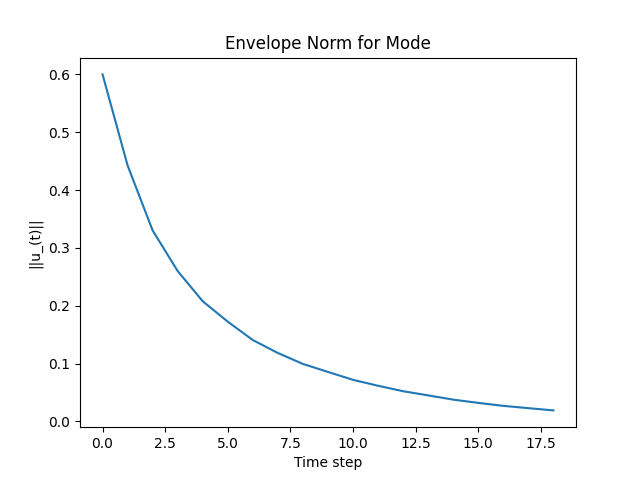
\includegraphics[width=\linewidth]{figs/interpret/envelope_norm_mode_long.png}
    \end{minipage}
\end{figure} \label{envelope_norm}


To validate the local linear approximation, at each \(k\) we sample \(N_{\rm trials}\) random perturbations \(\delta\in\mathbb{R}^{2H}\) of fixed norm \(\|\delta\|=\epsilon\), and compute:
\[
  r(\delta)
  = f\bigl((h_k,c_k)+\delta\bigr)
    - \Bigl[f(h_k,c_k) + J_k\,\delta\Bigr],
  \quad
  \varepsilon(\delta)
  = \frac{\|r(\delta)\|}{\|J_k\,\delta\|}.
\]
We report the empirical mean \(\mathbb{E}[\varepsilon]\) and maximum \(\max\varepsilon\) over trials.  Values \(\varepsilon\ll1\) indicate good first‐order accuracy, whereas values close to one reveal strong nonlinearity \ref{fig:error_rate}. 

\begin{figure}[h]
    \centering
    \begin{minipage}{0.49\textwidth}
        \centering
        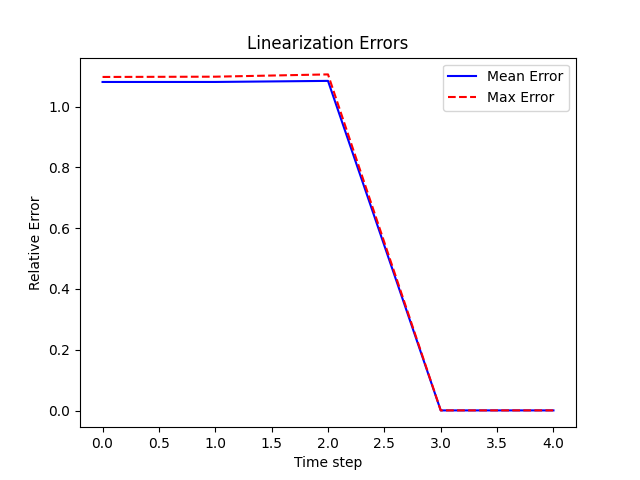
\includegraphics[width=\linewidth]{figs/interpret/linearization_errors_150.png}
    \end{minipage}
    \begin{minipage}{0.49\textwidth}
        \centering
        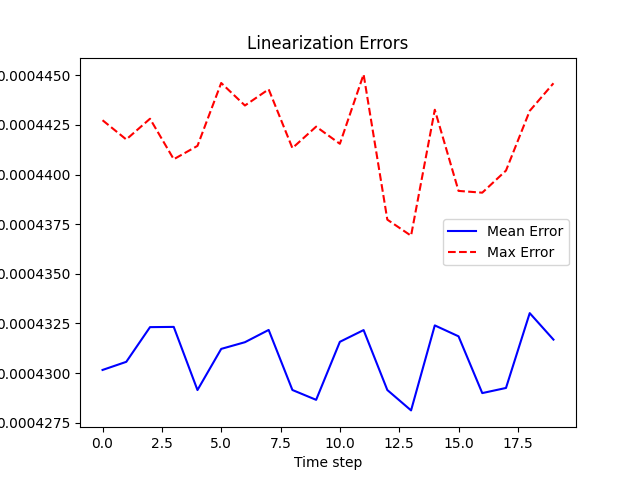
\includegraphics[width=\linewidth]{figs/interpret/linearization_errors_20.png}
    \end{minipage}
    \caption{Showcase the error rate of linear approximation for some times steps, as you can see the network dynamics eventually would have low error rate for linear approximation which cause network to converge to a a linear dynamics}
    \label{fig:error_rate}
\end{figure}


\section{Fourier‐Series Representability}

A real or complex-valued function $f(x)$ on $\mathbb{R}$ admits a Fourier series 
$$
f(x) \sim \sum_{n=-\infty}^{\infty} c_n e^{i 2 \pi nx / P}
$$
Provided it satisfies one of the standard convergence criteria below:
\begin{itemize}
    \item Dirichlet-Jordan conditions
    \item $L^2$ convergence and Carleson conditions
    \item Absolute and Uniform Convergence
\end{itemize}


\begin{definition}[The GCLSTM Estimator]
Let a GCLSTM network be a function that estimates a sequence of graphs. At each discrete time step $t \in \mathbb{N}$, the GCLSTM's internal state is a tuple $s_t = (h_t, c_t) \in \mathbb{R}^{2H}$, comprising a hidden state $h_t \in \mathbb{R}^H$ and a cell state $c_t \in \mathbb{R}^H$. The state transition is governed by a continuous function $f_{\text{cont}}$:
\begin{equation}
    s_{t+1} = (h_{t+1}, c_{t+1}) = f_{\text{cont}}(s_t, A_t)
\end{equation}
where $A_t$ is the adjacency matrix of the input graph at time $t$. The output is produced by a continuous decoder function, $\text{decoder}:\mathbb{R}^H \to \mathcal{O}$, where $\mathcal{O}$ is the output space (e.g., predicted graphs).
\end{definition}

\begin{remark}
For the scope of this analysis, we assume the GCLSTM is stable, i.e., its hidden and cell states do not experience exploding gradients and remain within a bounded subset of their respective spaces for any bounded input sequence. This is a standard assumption for any well-trained, practical recurrent model.
\end{remark}

\begin{definition}[The Signal for Analysis]
The primary signal for our analysis is the sequence of hidden states generated by the GCLSTM over a finite time horizon of $N$ steps. We denote this sequence as $\mathbf{h}$:
\begin{equation}
    \mathbf{h} = \{h_t\}_{t=0}^{N-1}, \quad \text{where } h_t \in \mathbb{R}^H
\end{equation}
\end{definition}

\begin{definition}[Discrete Fourier Transform (DFT)]
The DFT transforms the finite sequence $\mathbf{h}$ into a sequence of complex-valued vectors $\mathbf{H} = \{H_k\}_{k=0}^{N-1}$, where $H_k \in \mathbb{C}^H$. The $k$-th Fourier coefficient is defined by the finite sum:
\begin{equation}
    H_k = \sum_{t=0}^{N-1} h_t \cdot e^{-i \frac{2\pi k t}{N}}
\end{equation}
The Inverse DFT (IDFT) perfectly reconstructs the original sequence from its coefficients. As the DFT is a finite sum over a finite sequence, its existence and invertibility are guaranteed; classical convergence proofs are not required. Our goal is to prove that the signal $\mathbf{h}$ is sufficiently "well-behaved" for this transformation to be meaningful.
\end{definition}

\subsection{Required Conditions}

We now prove that the sequence $\mathbf{h}$ satisfies the discrete analogues of the three fundamental conditions for Fourier series representation.

\subsubsection{$L^2$ Condition: Finite Energy}
The continuous $L^2$ condition ensures a function has finite energy over its period. The discrete analogue for a sequence is membership in the $\ell^2$ space.

\begin{theorem}[Finite Energy of GCLSTM Sequences]
The hidden state sequence $\mathbf{h} = \{h_t\}_{t=0}^{N-1}$ from a stable GCLSTM has finite energy over any finite time horizon $N$.
\end{theorem}

\begin{proof}
The GCLSTM state update function $f_{\text{cont}}$ is composed of linear transformations and non-linear activation functions (e.g., $\tanh$, $\text{sigmoid}$). These activation functions are inherently bounded. For instance, for any input $x$, $|\tanh(x)| \le 1$ and $0 \le \text{sigmoid}(x) \le 1$.

Due to these bounded activations and the stability assumption, the state vectors $s_t$ are confined to a compact subset of $\mathbb{R}^{2H}$. Consequently, the Euclidean norm of any hidden state vector $h_t$ is bounded by some finite real constant $M > 0$:
\begin{equation}
    \|h_t\| \le M, \quad \forall t \in \{0, 1, \dots, N-1\}
\end{equation}
The total energy of the sequence $\mathbf{h}$, denoted $E(\mathbf{h})$, is the sum of the squared norms of its elements:
\begin{equation}
    E(\mathbf{h}) = \sum_{t=0}^{N-1} \|h_t\|^2
\end{equation}
Applying the bound from (4), we obtain:
\begin{equation}
    E(\mathbf{h}) \le \sum_{t=0}^{N-1} M^2 = N M^2
\end{equation}
Since both $N$ and $M$ are finite, it follows that $E(\mathbf{h}) < \infty$. Therefore, the sequence $\mathbf{h}$ is an element of the $\ell^2$ space over the finite interval $[0, N-1]$.
\end{proof}


\subsubsection{Dirichlet-Jordan Condition: Bounded Variation}
The Dirichlet-Jordan test requires a function to be of bounded variation, meaning it does not oscillate infinitely.

\begin{theorem}[Bounded Variation of GCLSTM Sequences]
The hidden state sequence $\mathbf{h} = \{h_t\}_{t=0}^{N-1}$ from a stable GCLSTM has bounded variation over any finite time horizon $N$.
\end{theorem}

\begin{proof}
The total variation, $V(\mathbf{h})$, of the discrete sequence $\mathbf{h}$ is defined as the sum of the norms of its first-order differences:
\begin{equation}
    V(\mathbf{h}) = \sum_{t=0}^{N-2} \|h_{t+1} - h_t\|
\end{equation}
The state update function $f_{\text{cont}}$ is continuous and, for a stable model, operates on a compact domain of state values. A continuous function on a compact set is Lipschitz continuous. This implies that the change between consecutive states is bounded. Therefore, there must exist a finite real constant $L > 0$ that bounds the norm of the difference between consecutive hidden states:
\begin{equation}
    \|h_{t+1} - h_t\| \le L, \quad \forall t \in \{0, 1, \dots, N-2\}
\end{equation}
Using this bound, we can establish an upper bound for the total variation:
\begin{equation}
    V(\mathbf{h}) \le \sum_{t=0}^{N-2} L = (N-1)L
\end{equation}
As $N$ and $L$ are finite, we have $V(\mathbf{h}) < \infty$. The sequence $\mathbf{h}$ is thus of bounded variation.
\end{proof}


\subsubsection{Uniform Convergence Condition: Discrete Smoothness}
In the continuous domain, function continuity is a key prerequisite for uniform convergence of its Fourier series. The discrete analogue relates to the regularity and predictability of the sequence from one step to the next.

\begin{proposition}[Step-wise Continuity of GCLSTM Sequences]
The GCLSTM architecture imposes a step-wise continuity on its hidden state sequence, which serves as the discrete analogue of function continuity.
\end{proposition}

\begin{proof}
By Definition 2.1, the state update function $f_{\text{cont}}$ is continuous with respect to its arguments, $s_t$ and $A_t$. For a given input sequence $\{A_t\}$, the mapping from state $s_t$ to $s_{t+1}$ is continuous. This ensures that the sequence $\mathbf{h}$ is non-pathological; it does not contain arbitrary or infinite jumps. A small perturbation in the state $s_t$ will result in a correspondingly small perturbation in the state $s_{t+1}$. This regularity is the discrete counterpart to the smoothness properties that ensure well-behaved convergence in continuous-time Fourier analysis.
\end{proof}


We have formally demonstrated that finite-length sequences of hidden states generated by a stable GCLSTM network satisfy the discrete analogues of the primary conditions required for Fourier series representation. Specifically, we have proven that such sequences possess finite energy (are in $\ell^2$), are of bounded variation, and exhibit step-wise continuity. These properties ensure that the Discrete Fourier Transform is not only a well-defined operation on these sequences but also a meaningful tool for analyzing the temporal and periodic patterns learned by complex graph recurrent neural networks. This theoretical validation supports the application of spectral methods in the study and interpretation of dynamic graph models that we establish in the subsequent sections.



\subsection{Fourier-Spectral Analysis}

On top of analysis in previous section we perform a classical signal-processing probe on GCLSTM's hidden-state time series. Our goal is to detect any sustained oscillatory components at the idea AABB frequencies.

Given the hidden‐state trajectory
\[
  H_{\rm traj}
  = \bigl[h_0,\;h_1,\;\dots,\;h_{T_{\rm tot}-1}\bigr]^\top
  \;\in\;\mathbb{R}^{T_{\rm tot}\times H},
\]
we compute the DFT along the temporal axis, component‐wise:
\[
  Y(f,j)
  = \sum_{t=0}^{T_{\rm tot}-1}
    \bigl[H_{\rm traj}(t,j)\bigr]\,
    e^{-\,i2\pi f\,t/T_{\rm tot}},
  \quad f = 0,1,\dots,\lfloor T_{\rm tot}/2\rfloor,
\]
where \(j=1,\dots,H\) indexes hidden‐units and \(f\) is the discrete frequency bin.  This is the standard periodogram estimator of the spectrum \citep{OppenheimSchaferDSP,StoicaMosesSpectral}.

We then form the average power spectral density across units:
\[
  \mathrm{PSD}(f)
  = \frac{1}{H}
    \sum_{j=1}^{H} \bigl|Y(f,j)\bigr|^2.
\]
Peaks in \(\mathrm{PSD}(f)\) correspond to strong periodic components in the hidden‐state.  In a perfectly undamped AABB clock, one expects Dirac‐like lines at
\[
  f = \frac{1}{4}\quad\text{and/or}\quad f=\frac{1}{2}
  \quad\text{(cycles per time step)},
\]
since the pattern repeats every 4 steps. From this analysis we expect to see:
\begin{itemize}
    \item Sharp, PSD peak at \(f=0.25\) (and/or \(f=0.5\)) indicates a persistent oscillation in the hidden‐state, i.e.\ a unit‐modulus Floquet mode in disguise.
    \item A low-frequency hump or small side-lobes reveals only transient or noisy periodic, consistent with damped modes $|\lambda| < 1$.
    \item Absence of peaks confirms that the network did not learn and undamped internal clock, but rather a decaying, input-driven signal.
\end{itemize}
As shown in Fig \ref{fig:fourier} the spectrum has a dominant low frequency hump new $f \approx 0$ and no sharp peak at $f = 0.25, 0.5$ cycles. These observation agaib strength the hypothesis about undamped oscillation in hidden-state of GCLSTM, and how this model "re-encode" instead of learning the frequencies.


\begin{figure}[h]
    \centering
    \begin{minipage}{0.49\textwidth}
        \centering
        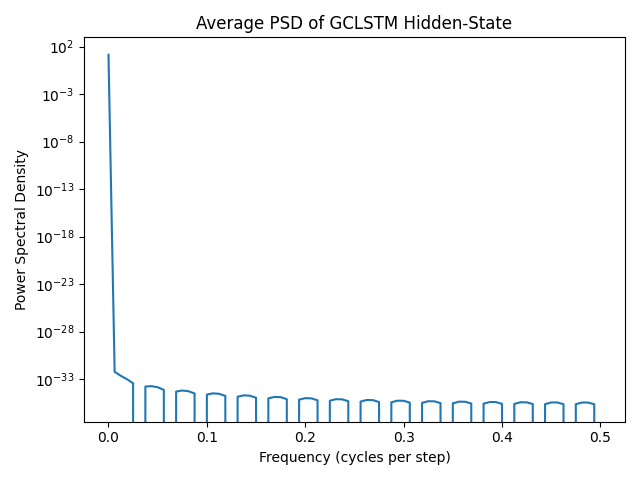
\includegraphics[width=\linewidth]{figs/interpret/floquet_frequencies_PSD.png}
    \end{minipage}
    \caption{PSD of Fourier transformation on full hidden-state time series matrix \(H_{\rm traj}\in\mathbb{R}^{T_{\rm tot}\times H}\) (\(T_{\rm tot}=160\))} 
    \label{fig:fourier}
\end{figure}


We also did PCA visualization of $H_{\textit{traj}}$ in 3D, project the matrix into its left eigenvectors, based on previous results we expect:
\begin{itemize}
    \item A closed loop (approximately circular) in PCA space is indication of a smooth, nonlinear periodic orbit \cite{Mezić2013Koopman}.
    \item A zig-zag (line-segment bounce) indicates that the hidden-state moves back and forth between two or more distinct clusters without sweeping our a continuous cycle. This is typical when the network re-encodes the pattern discretely at each step but dose not interpolate smoothly between them \ref{fig:pca} .
\end{itemize}

\begin{figure}[h]
    \centering
    \begin{minipage}{0.49\textwidth}
        \centering
        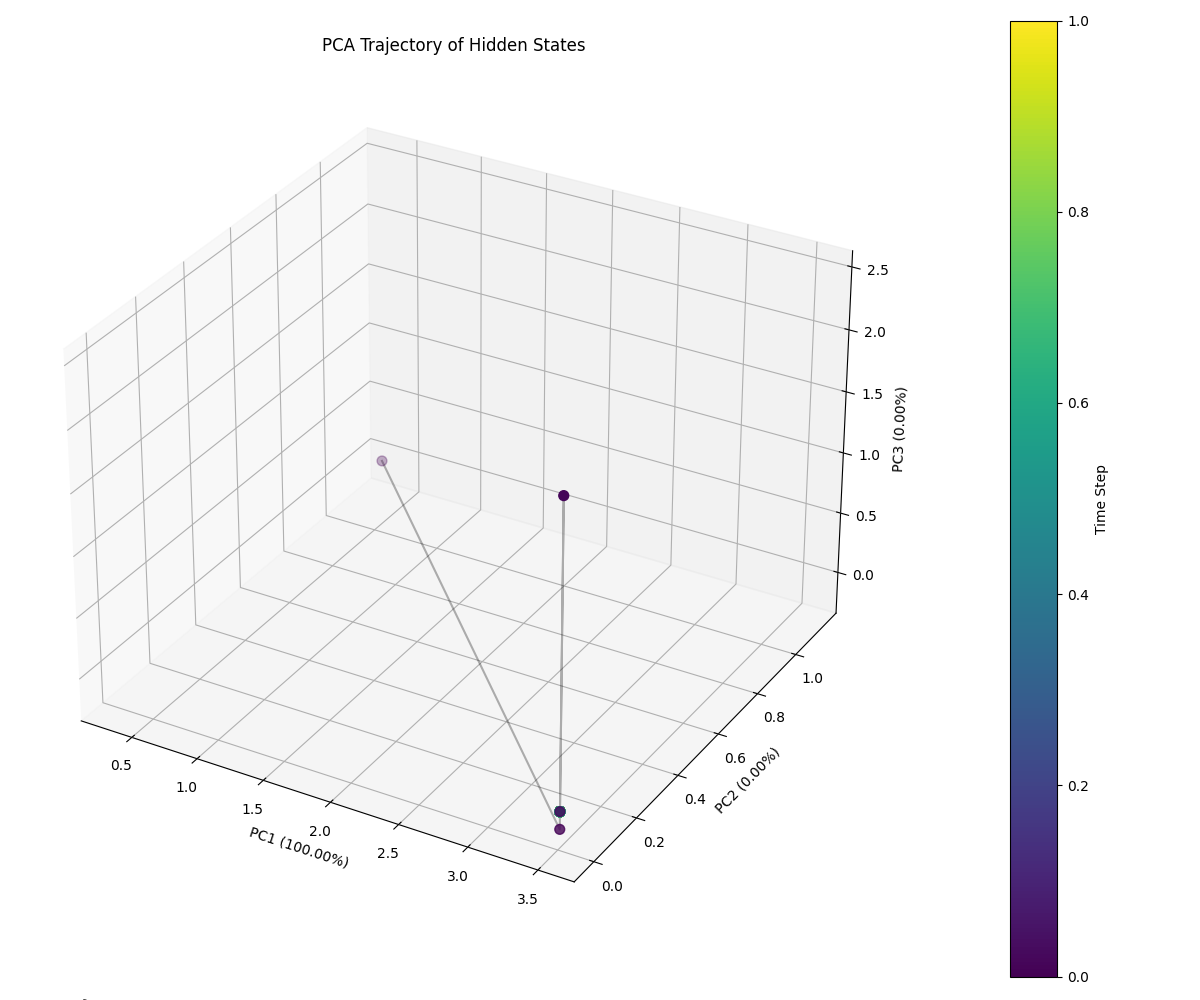
\includegraphics[width=\linewidth]{figs/interpret/hidden_state_pca_trajectory.png}
    \end{minipage}
    \caption{PCA visualization of full hidden full hidden-state time series matrix \(H_{\rm traj}\in\mathbb{R}^{T_{\rm tot}\times H}\) (\(T_{\rm tot}=160\))} 
    \label{fig:pca}
\end{figure}

\subsubsection{Interpretations}
Together, these additional analysis demonstrate that GCLSTM does not maintain an undamped periodic subspace (clock-modes). Rather, it continually re-encodes the current A vs. B phase from the input and allows that signal to decay, reproducing the characteristic $F_1$-score dips and recoveries at each replication period \ref{fig:(2,N)_perday}, this can explain the forgetting like behavior shown in the Fig \ref{fig:(2,N)_perday}.



% \section{Toy example}

% \subsection{Embedding the GCLSTM Recurrence into a Periodic Linear ODE}

% We have seen that, along the reference AABB orbit, a GCLSTM’s discrete dynamics can be linearized at each integer time \(k\) by the Jacobian
% \[
%   J_k \;=\;\frac{\partial\,(h_{k+1},c_{k+1})}{\partial\,(h_k,c_k)}\;\in\;\R^{2H\times2H},
%   \quad k=0,1,2,3,
% \]
% and that the one‐period map
% \[
%   J_{\rm cycle}
%   = J_3\,J_2\,J_1\,J_0
% \]
% yields the Floquet multipliers of the discrete‐time system.  We now show that exactly the same monodromy appears as the Poincaré map of a continuous, \emph{piecewise‐constant} linear ODE of the form
% \[
%   \dot x(t) \;=\; A(t)\,x(t),
%   \qquad
%   A(t+4)=A(t),
%   \quad
%   A(t)\in\R^{2H\times2H}.
% \]

% \medskip
% \paragraph{1. Definition of the piecewise‐constant generator \(A(t)\).}
% Partition time into intervals \([k,k+1)\), \(k\in\Z\).  On each interval we set
% \[
%   A(t) \;=\; A_k,
%   \quad
%   t\in[k,k+1),
%   \quad
%   A_k \;=\;\log\!\bigl(J_k\bigr)\;\in\;\R^{2H\times2H},
% \]
% where \(\log\) denotes any branch of the matrix logarithm (existence guaranteed because \(J_k\) is real‐invertible with no negative real eigenvalues, as seen empirically).  By construction \(A(t+4)=A(t)\), so \(A(t)\) is \(4\)‐periodic.

% \medskip
% \paragraph{2. Solution operator and monodromy.}
% On each interval \([k,k+1)\) the ODE \(\dot x = A_k x\) has fundamental solution
% \[
%   \Phi(t,k)\;=\;\exp\!\bigl((t-k)\,A_k\bigr),
%   \quad t\in[k,k+1].
% \]
% Hence over one unit step,
% \[
%   x(k+1) \;=\;\Phi(k+1,k)\,x(k)
%   \;=\;\exp\!\bigl(A_k\bigr)\,x(k)
%   \;=\;J_k\,x(k).
% \]
% Chaining four intervals,
% \[
%   x(4) \;=\;
%   J_3\,J_2\,J_1\,J_0\,x(0)
%   \;=\;J_{\rm cycle}\,x(0).
% \]
% Thus the continuous‐time ODE’s Poincaré (one‐period) map
% \(\Phi(4,0)\) exactly matches the discrete monodromy \(J_{\rm cycle}\).

% \medskip
% \paragraph{3. Equivalence and Floquet analysis.}
% Since \(\Phi(t+4,0)=\Phi(t,0)\,\Phi(4,0)\), classical Floquet theory for continuous‐time linear systems applies: the eigenpairs of \(\Phi(4,0)\) are the Floquet multipliers and modes, and one constructs \(T\)-periodic envelopes \(u_j(t)\) satisfying
% \[
%   \Phi(t,0)\,v_j = e^{\mu_j\,t}\,u_j(t),
%   \quad
%   u_j(t+4)=u_j(t),
%   \quad
%   \mu_j=\tfrac1{4}\ln(\lambda_j).
% \]
% But \(\Phi(4,0)=J_{\rm cycle}\), so all eigenvalues \(\lambda_j\) and eigenvectors \(v_j\) coincide with those we extracted from the discrete Jacobian product.  Likewise, the envelope
% \(\;u_j(t)=\Phi(t,0)\,v_j\) restricted to integer \(t\) agrees with
% \(\;J_{t-1}\cdots J_0\,v_j\).

% \medskip
% \paragraph{4. Summary of the formal equivalence.}
% \begin{enumerate}
%   \item \textbf{Discrete model:} 
%   \(\;s_{k+1}=f(s_k)\), linearized to \(\;s_{k+1}-s_{k+1}^*\approx J_k\,(s_k-s_k^*)\).  
%   \item \textbf{Continuous embedding:} 
%   \(\;\dot x(t)=A(t)\,x(t)\) with \(A(t)=\log(J_{\lfloor t\rfloor})\).  
%   \item \textbf{One‐period map:} 
%   \[
%     \Phi(4,0)=\prod_{k=0}^{3}\exp(A_k)
%     =\prod_{k=0}^{3}J_k = J_{\rm cycle}.
%   \]
%   \item \textbf{Floquet theory:}  
%   Both discrete and continuous formulations yield the same Floquet multipliers \(\lambda_j\), exponents \(\mu_j\), and envelopes \(u_j(t)\).
% \end{enumerate}

% \noindent Hence all of our prior Floquet‐mode, envelope‐reconstruction, and spectral analyses carry over verbatim in the ODE framework \(\dot x=A(t)x\), providing a unified continuous‐ and discrete‐time perspective on how the GCLSTM encodes (and decays) periodic graph sequences.



\bibliographystyle{plain} % We choose the "plain" reference style
\bibliography{ref.bib} % Entries are in the refs.bib file

\end{document}


